%%%%%%%%%%%%%%%%%%%%%%%%%%
% Document configuration %
%%%%%%%%%%%%%%%%%%%%%%%%%%

\documentclass[
aspectratio=169,
bigger,
xcolor=table,
]{beamer}

\usepackage[french]{babel}
\usepackage{
	palettechum,
	n,
	pgfplots,
	emoji,
	wasysym,
	servou,
	colortbl,
	beamer-progress,
}
\usepackage[
	backend=biber,
	autolang=none,
	style=authoryear,
	doi=false,
%	url=false,
	isbn=false
]{biblatex}


\usetheme{viger}
\usetikzlibrary{spy, matrix}
\usepgfplotslibrary{groupplots}

\setbeamertemplate{footline}[progress bar]
\setbeamertemplate{frametitle continuation}[from second]
\setbeamercovered{transparent=50}
\pgfplotsset{
	compat=newest,
	tickwidth=1mm,
	every axis/.style={
		fg!65,
		minor x tick num=1,
		axis lines*=left,
		cycle list={
			{turquoisechum}
		},
		grid style={fg!30!bg, dotted},
		grid=both,
		font=\tiny,
		no markers,
		enlargelimits=false,
		xlabel=Temps (s),
		width=\textwidth, 
		height=0.45\textheight,
	},
	every axis plot/.style={
		line width=0.5pt,
	}
}


\defbibheading{bibliography}[\bibname]{}
\AtBeginSection{
	\begin{frame}{Plan}
		\tableofcontents[currentsection]
	\end{frame}
}

\def\chm{cm\,H\textsubscript{2}O}
%%%%%%%%%%%%%%%%%%%%
% Meta-information %
%%%%%%%%%%%%%%%%%%%%

\title{Ventilation: quand le coeur s'en mêle ...\emoji{beating-heart}}
\author{\ninh}
\institute{\qhum}

\addbibresource{autotriggering.bib}

%%%%%%%%%%%
% Content %
%%%%%%%%%%%

\begin{document}

\input{sectionPréambule}
\begin{frame}{Discussion}
	\begin{itemize}
		\item Avez-vous déjà été témoin d'un autodéclenchement ?
		\item Comment vous en êtes-vous rendu compte ?
		\item Quelle est votre \emph{recette} pour ajuster le seuil de
			déclenchement ?
	\end{itemize}
\end{frame}
\section{Histoire cas}

\begin{frame}{Histoire de cas}
	\centering
	\begin{columns}
		\column{0.49\textwidth}
		\begin{itemize}
			\item Homme de 68 ans
			\item Fibrose pulmonaire idiopathique
			\item Greffe pulmonaire unilatérale
			\item Embolie pulmonaire, sepsis...
			\item Réintubé pour bronchoscopie
		\end{itemize}
		\column{0.49\textwidth}
	\centering
			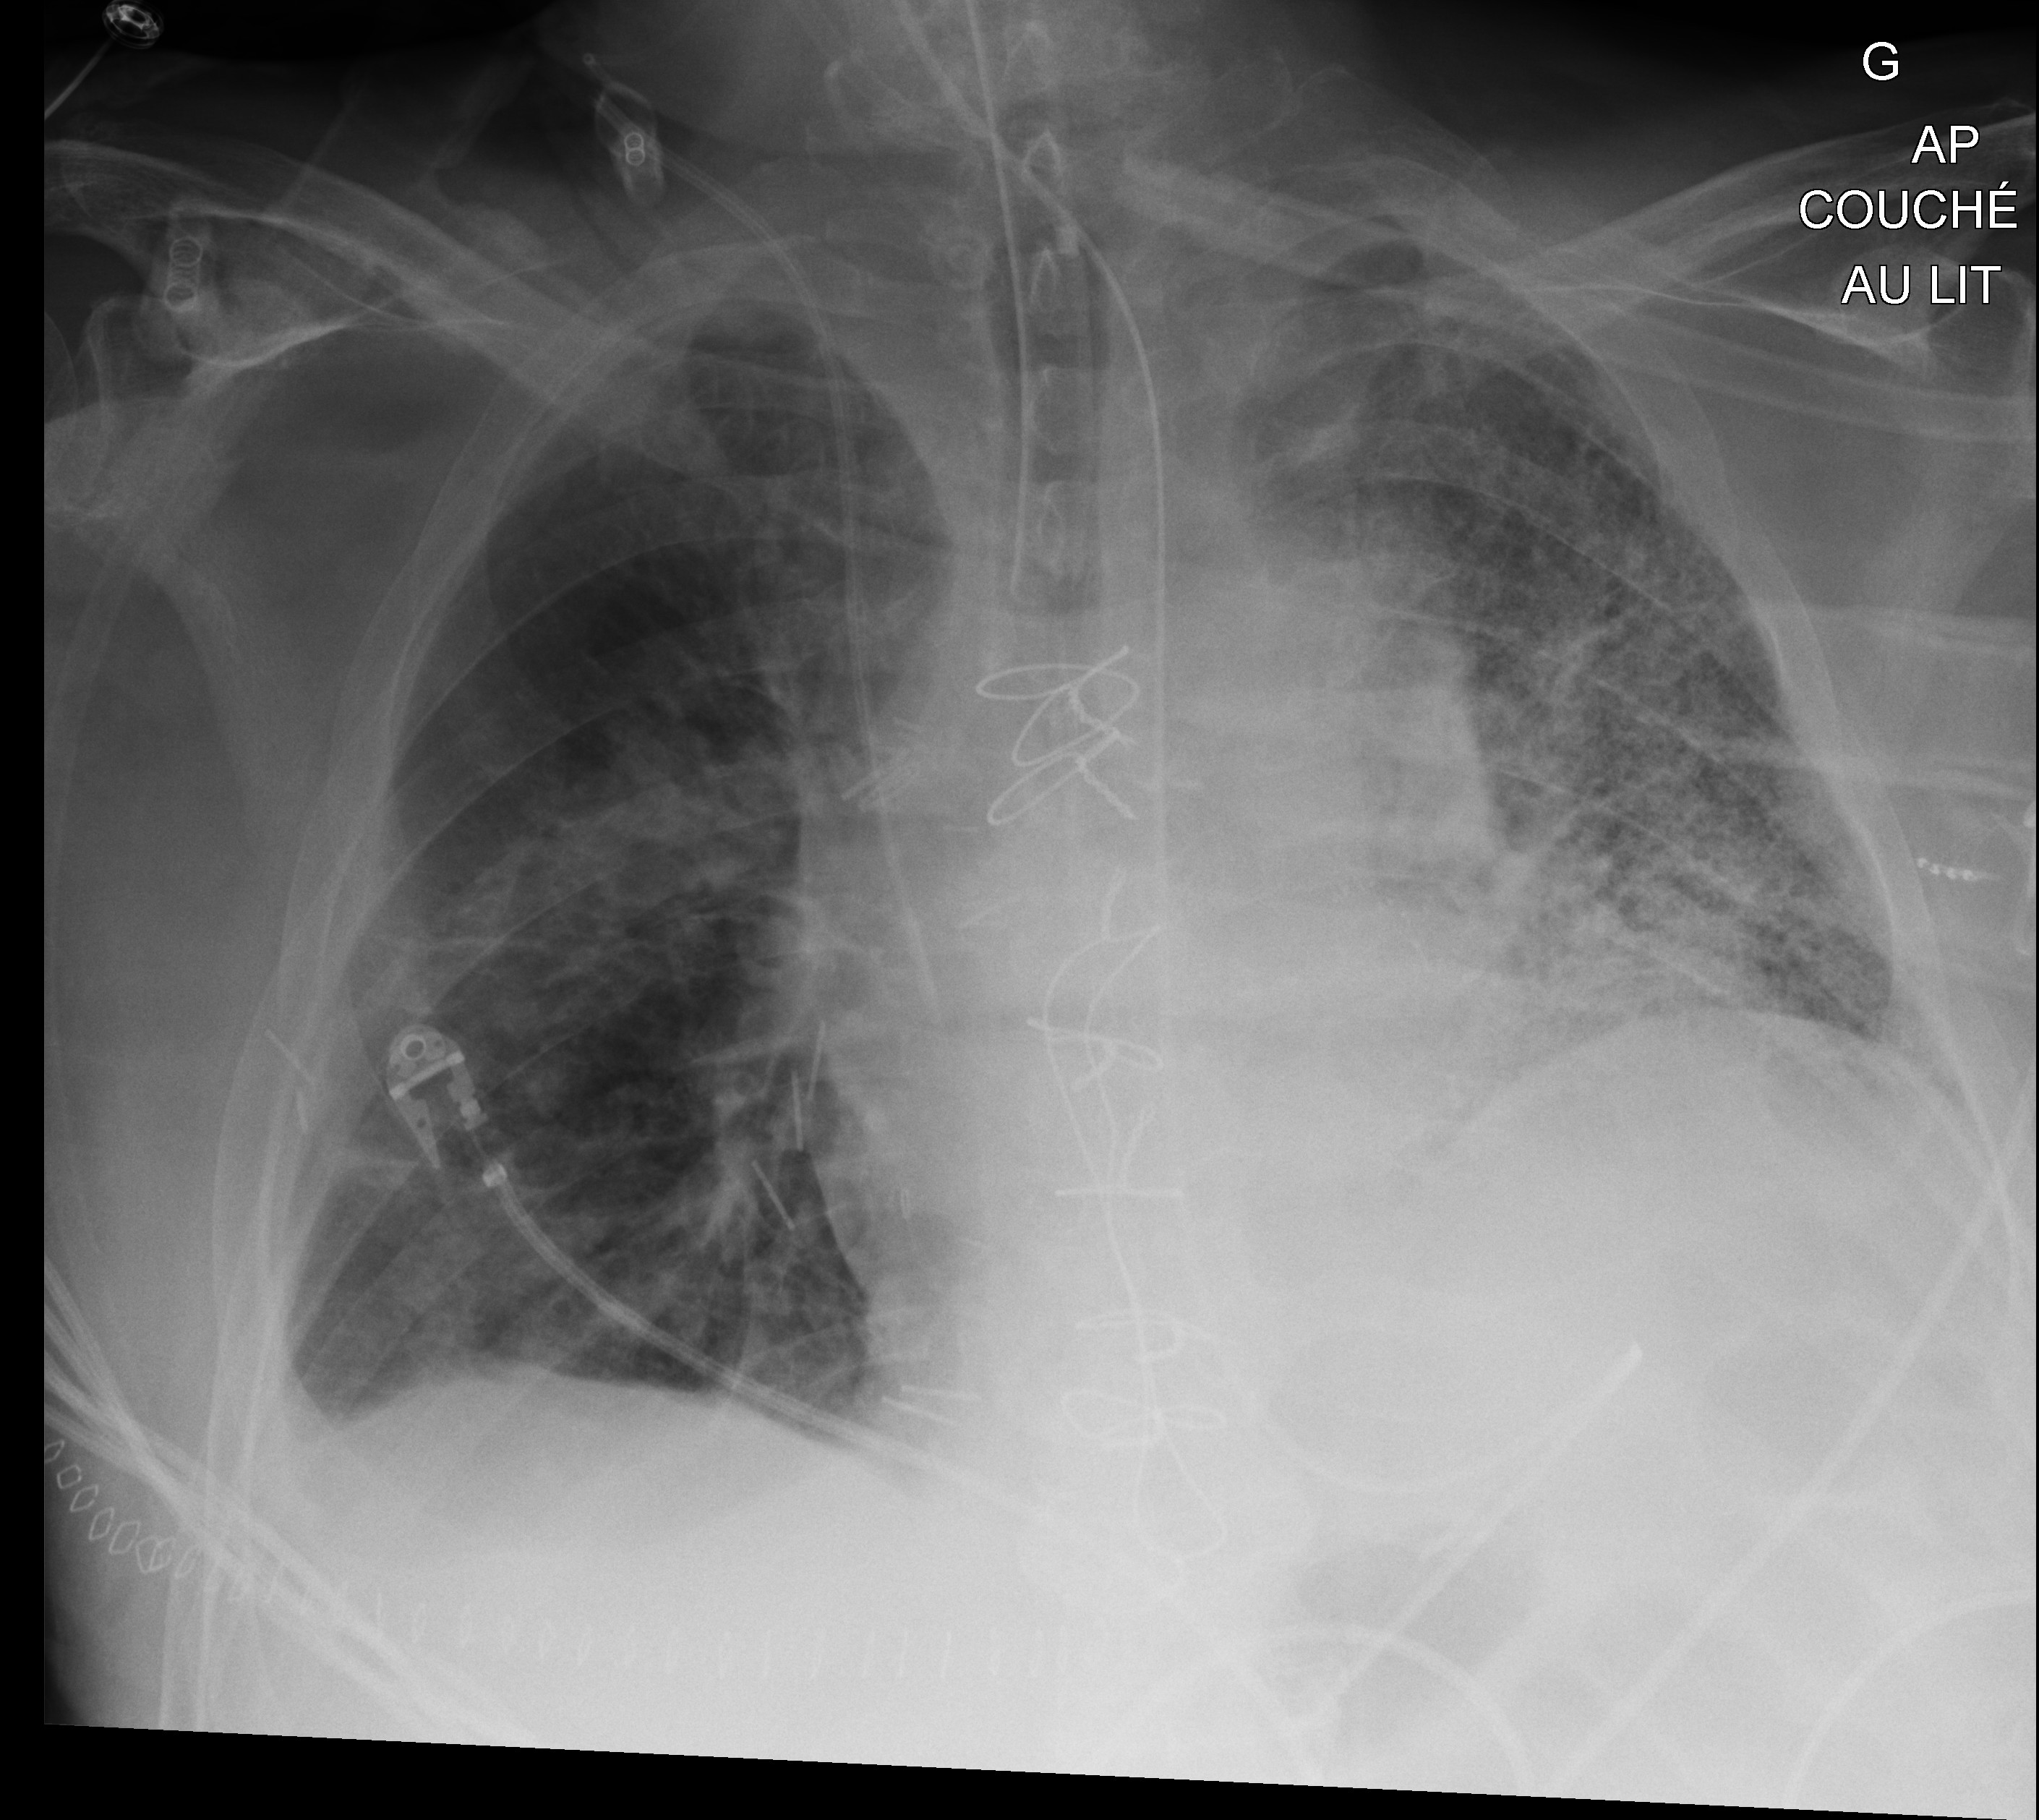
\includegraphics[
			width=\textwidth,
			trim=200 250 0 0,
			clip
			]{radiographies/23marsPM.jpg}
\end{columns}
\end{frame}

\begin{frame}
	\centering
	\begin{tikzpicture}
		\node[inner sep=0] (R) { 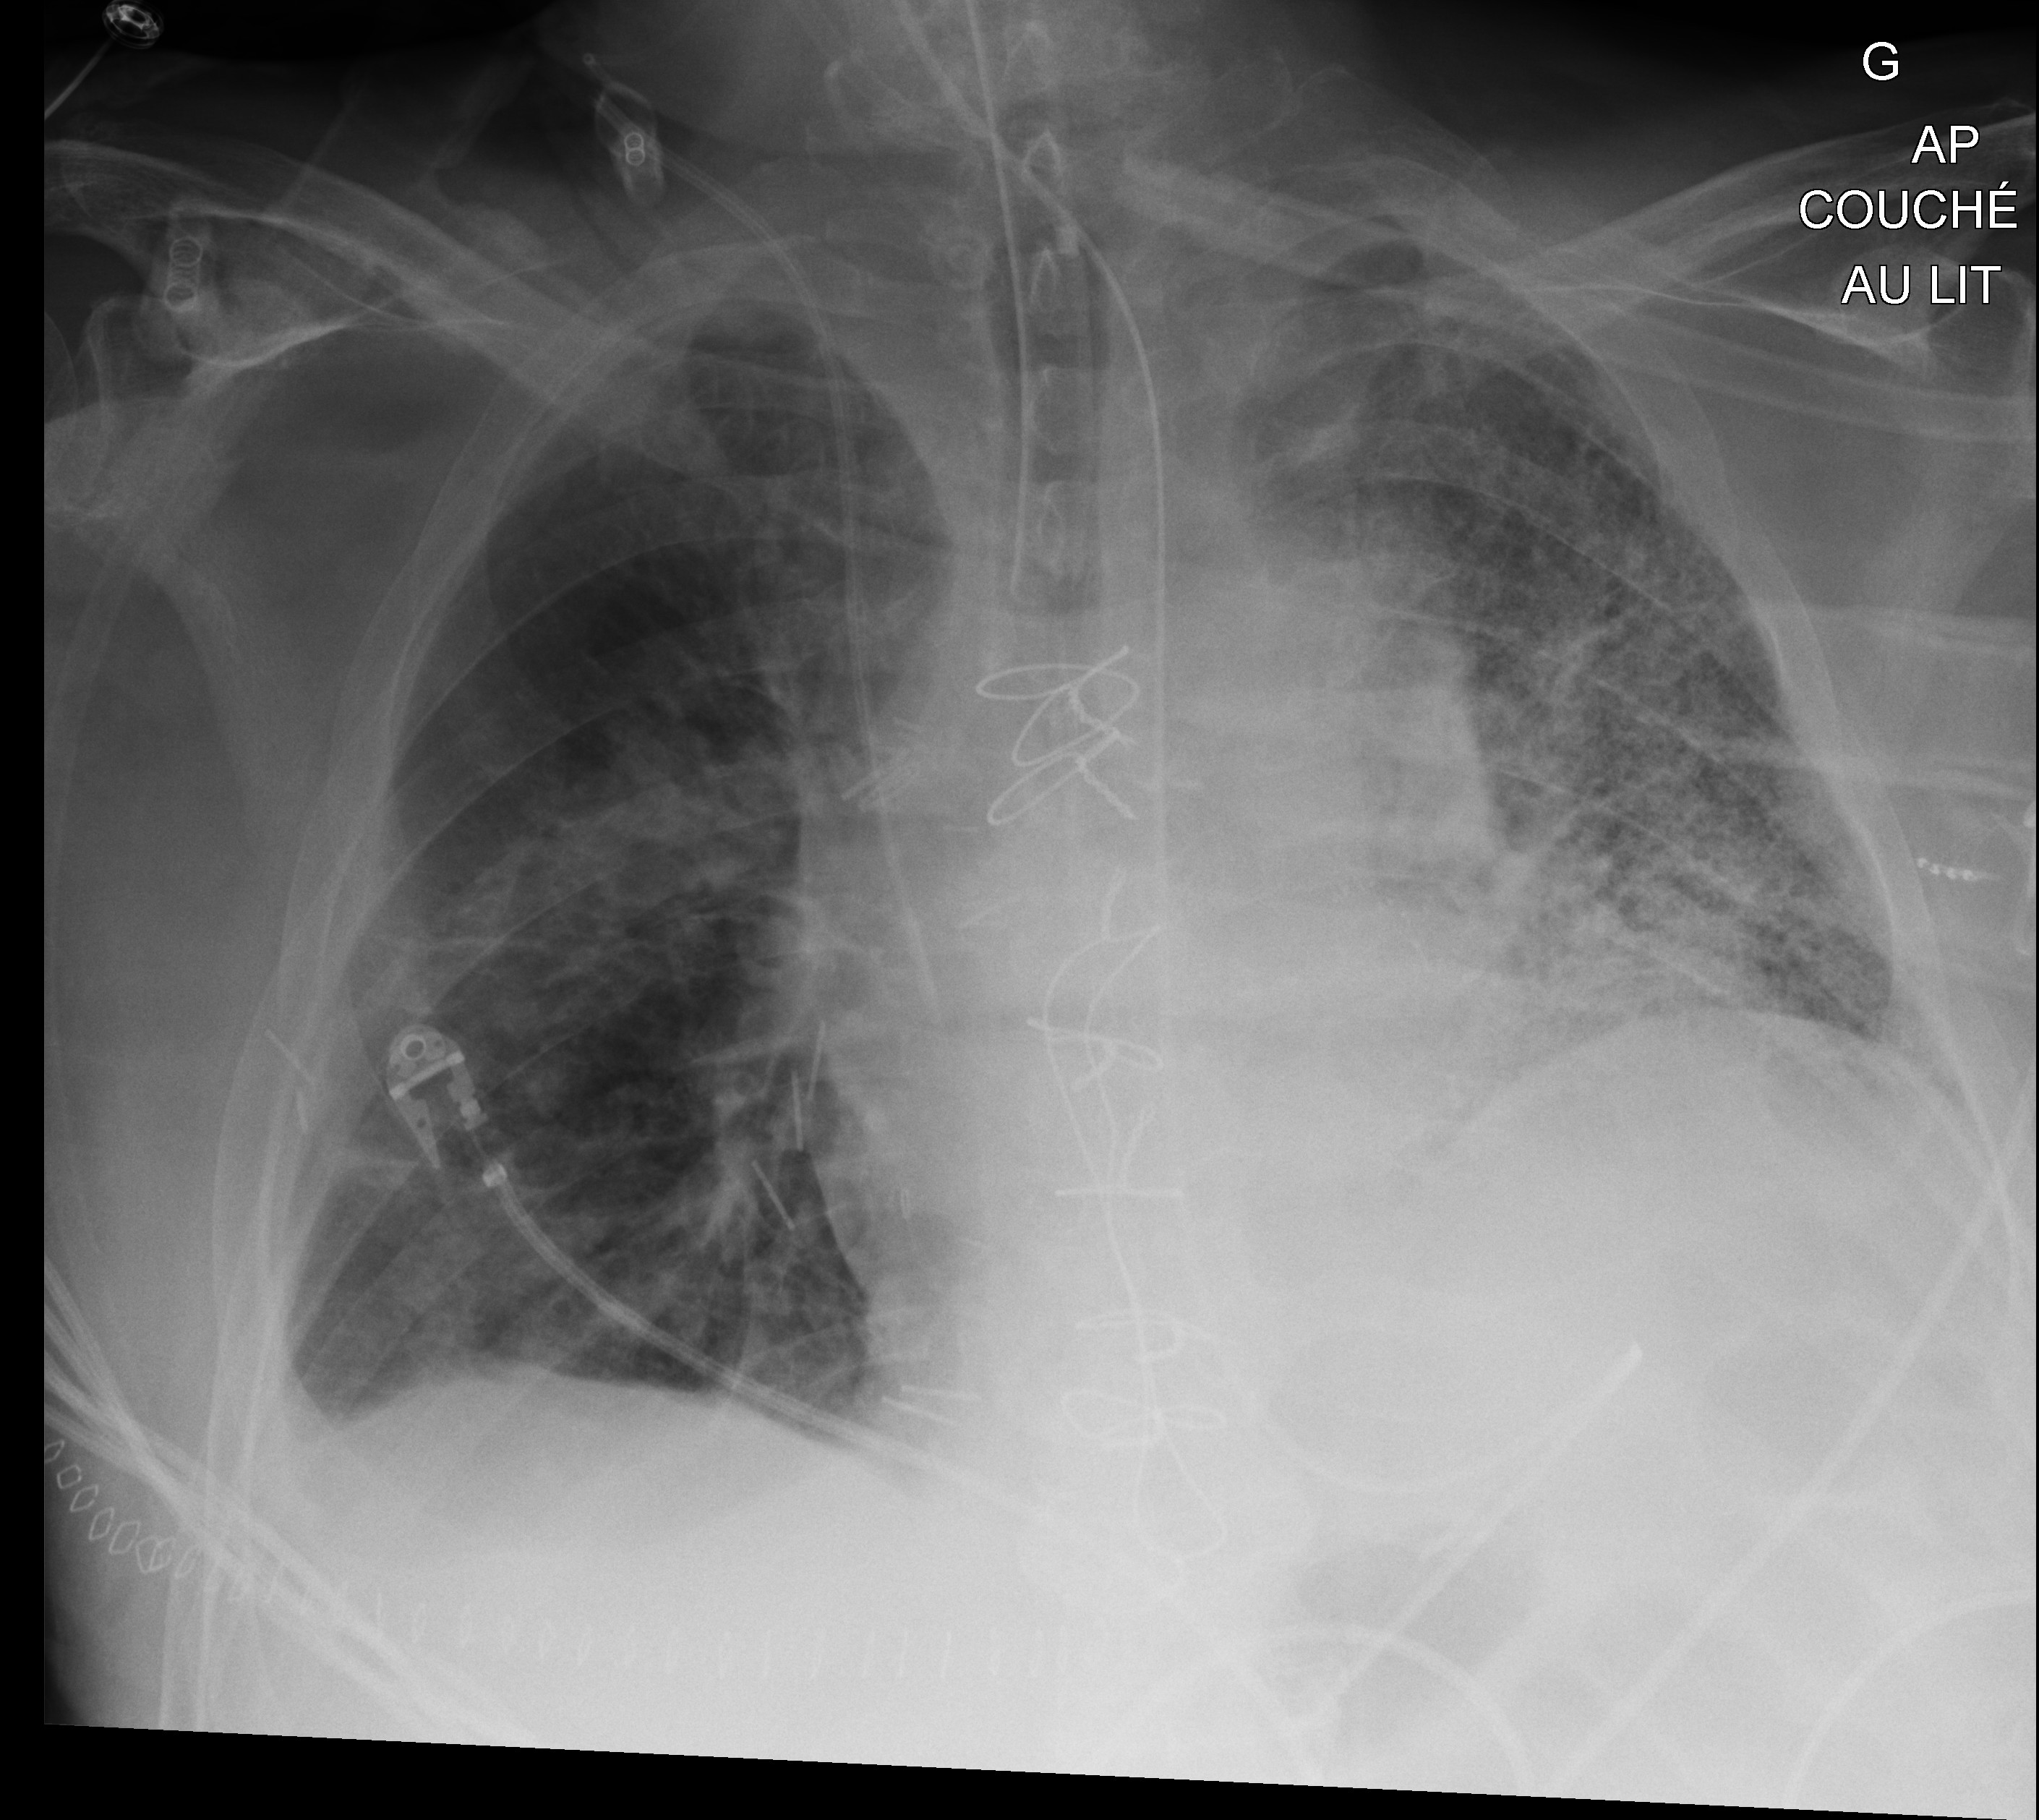
\includegraphics[
			height=\paperheight-1mm,
			trim=200 250 0 0,
			clip
			]{radiographies/23marsPM.jpg}
		};
		\end{tikzpicture}
\end{frame}

%%%%%%%%%%%%%%%%%%%%%%%%%%%%%%%%%%
% Chronologie                    %
%%%%%%%%%%%%%%%%%%%%%%%%%%%%%%%%%%

\begin{frame}{Chronologie}
	\centering

	\begin{tikzpicture}[
		xscale=0.4,
		pin distance=9mm,
		every node/.style={
			fill,
			circle,
			inner sep=1.5pt
		},
		every pin/.style={
			rectangle,
			text=bleuclairchum,
			fill=none
		},
		grad/.style={
			fill=none,
			label=below:j.\,\x,
			font=\tiny
		}
		]

		\draw [->](-1, 0) -- (29, 0);

		\begin{scope}[
			fill=bleuclairchum
		]
		\node [pin=Greffe pulmonaire, label=below:j.\,0] at(0, 0) {};
		\node [pin=below:Extubation, label=above:j.\,1] at(1, 0) {};
		\node [pin=Intubation, label=below:j.\,11] at(11, 0) {};
		\node [pin=below:Extubation, label=above:j.\,15] at(15, 0) {};
		\node [pin=Intubation, label=below:j.\,22] at(22, 0) {};
		\node [pin=below:Découv. autocécl., label=above left:j.\,25] at(25, 0) {};
		\node [pin={[text=red]below:Découv. autocécl.}] at(25, 0) {};
		\node [pin={[pin distance=1.5cm]Extubation}, label=below right:j.\,26] at(26, 0) {};
	\end{scope}
	\end{tikzpicture}

\end{frame}
%%%%%%%%%%%%%%%%%%%%%%%%%%%%%%%%%
% Captures d'écran              %
%%%%%%%%%%%%%%%%%%%%%%%%%%%%%%%%%

\begin{frame}
	\centering
	\begin{tikzpicture}[
		spy using outlines={circle,
      magnification=4,
			connect spies
		},
		servoucell/.append style={
			fill=black!80,
			text=white, 
			transform shape,
			scale=0.5
		}
	]
	\node [inner sep=0] (img) {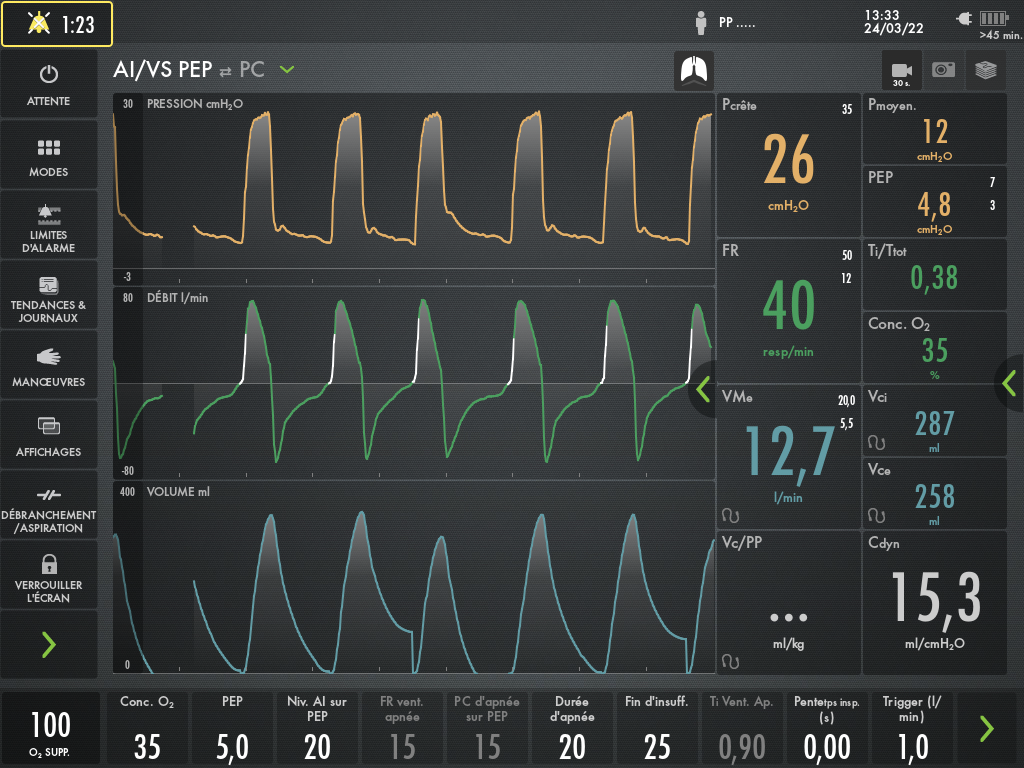
\includegraphics[height=\pageheight]{captures/220324_133316.png}};
	\only<2>\spy[red, size=3cm] on (-.2,0) in node at (2,2);
	\only<3>\spy[red, size=3cm] on (-.1,1.8) in node at (-3,2);
\node<4>[servoucell, anchor=west] at(img.east){
		\nodepart{one}P0.1
			\nodepart[font=\Huge]{two}0.2
				\nodepart{three}cm\,H\scalebox{.75}{2}O
				};
	\end{tikzpicture}
\end{frame}


\begin{frame}
	\centering
			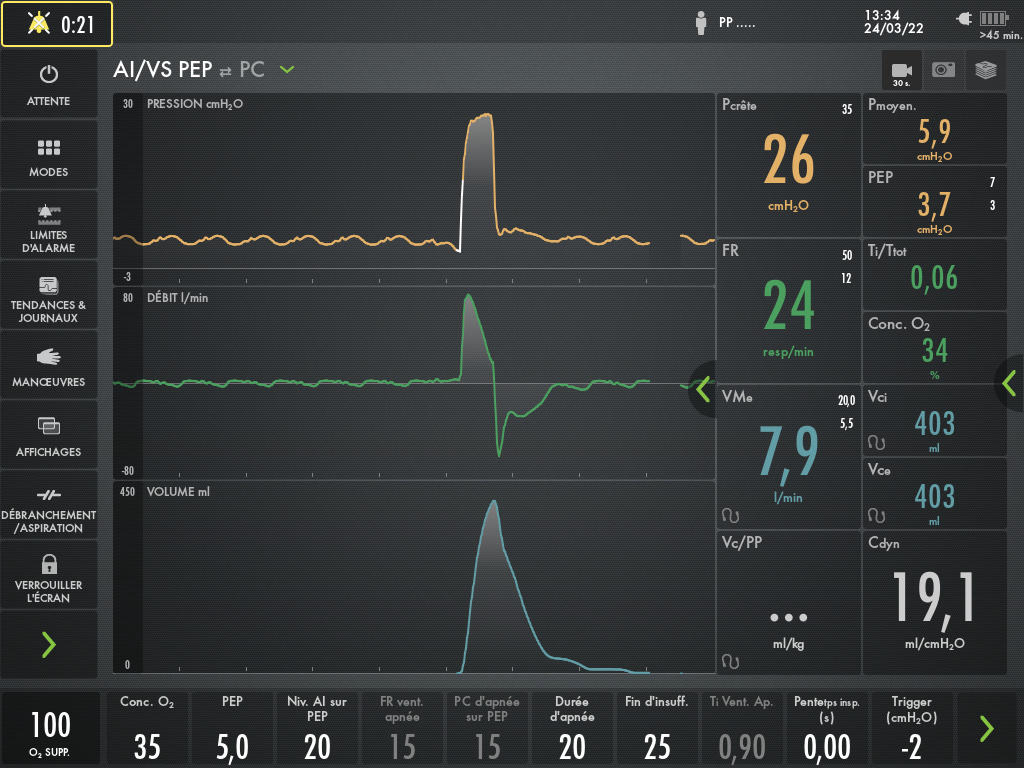
\includegraphics[height=\pageheight]{captures/220324_133418.png}
\end{frame}

\begin{frame}
	\centering
	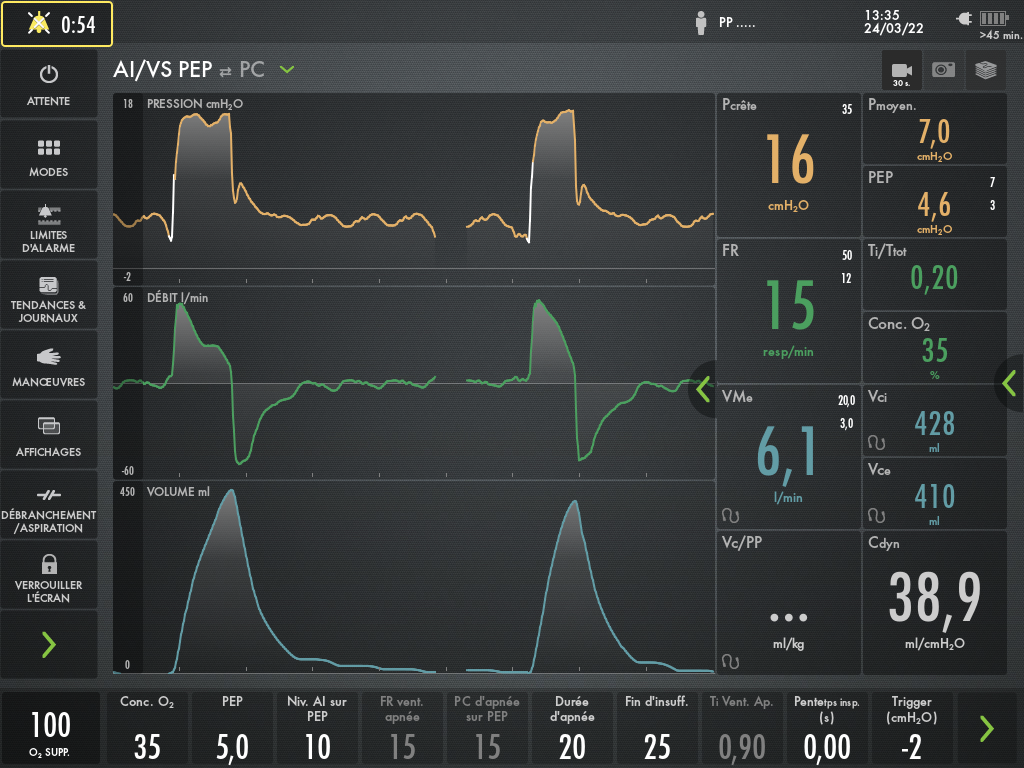
\includegraphics[height=\pageheight]{captures/220324_133546.png}
\end{frame}


%%%%%%%%%%%%%%%%%%%%%%%%%%%%%%%%%
% Traçés                        %
%%%%%%%%%%%%%%%%%%%%%%%%%%%%%%%%%

\section{Analyse du phénomène}


\def\zoomedplot{%
	\begin{tikzpicture}

		\begin{groupplot}[
			group style={
				group size=1 by 2,
				xlabels at=edge bottom,
			},
			height=0.35\textheight,
			width=0.6\textwidth,
			xlabel=Temps (s),
			xmin=2.5,
			xmax=9,
			]

			\nextgroupplot[ylabel=Pression (hPa)]
			\addplot [vertchum] table[x index=0, y index=2] {data/1648128876436-parsed.dat};

			\nextgroupplot[ylabel=Débit (l/m)]
			\addplot [bleuclairchum] table[x index=0, y index=3] {data/1648128876436-parsed.dat};

		\end{groupplot}
	\end{tikzpicture}
}

\begin{frame}
	\begin{tikzpicture}[
		highlight/.style={
			fill=white,
			opacity=0.3
		}
		]

		\begin{groupplot}[
			group style={
				group size=1 by 2,
				xlabels at=edge bottom,
			},
			height=0.40\textheight,
			xlabel=Temps (s),
			]

			\nextgroupplot[ylabel=Pression (hPa)]
			\addplot [vertchum] table[x index=0, y index=2] {data/1648128876436-parsed.dat};
			\fill<2> [highlight] (2,0) rectangle (9,\pgfkeysvalueof{/pgfplots/ymax});

			\nextgroupplot[ylabel=Débit (l/m)]
			\addplot [bleuclairchum] table[x index=0, y index=3] {data/1648128876436-parsed.dat};
			\fill<2> [highlight] (2,\pgfkeysvalueof{/pgfplots/ymin}) rectangle (9,\pgfkeysvalueof{/pgfplots/ymax});

		\end{groupplot}
		\node<2> [
			draw,
			fill=marinechum!20!black,
			] at(9,-1) {\zoomedplot};
	\end{tikzpicture}
\end{frame}

\usetikzlibrary{graphs, graphdrawing}
\usegdlibrary{trees}

\def\datadi{"data/1628779222908-parsed.dat"}
\def\datadchf{"data/1648112239967-parsed.dat"}
\def\adcbf{captures/screenshot_2022-04-02_09-59-56-waveforms.png}

\def\figad#1{%
	\begin{tikzpicture}

		\begin{groupplot}[
			group style={
				group size=1 by 2,
				xlabels at=edge bottom,
			},
			height=0.40\textheight,
			xlabel=Temps (s),
			]

			\nextgroupplot[ymin=0,ylabel=Pression (hPa)]
			\addplot [vertchum] table[x index=0, y index=2] {#1};

			\nextgroupplot[ylabel=Débit (l/m)]
			\addplot [bleuclairchum] table[x index=0, y index=3] {#1};

		\end{groupplot}
	\end{tikzpicture}
}

\def\figadchf{%
	\figad{\datadchf}
}
\def\figadi{%
	\figad{\datadi}
}

\begin{frame}{Classification de Nicolas\footnote{Publié dans \emph{aucune} revue prestigieuse}}
	\centering
\begin{tikzpicture}[
		anchor=west,
		grow'=right,
		child anchor=west,
		level distance=0mm,
		sibling distance=1.1cm,
		every node/.style={
			fill=vertchum,
			draw=black,
			text=black,
			yshift=-1.8cm,
			rounded corners,
			inner sep=2mm
		},
		edge from parent path= {(\tikzparentnode.-160) |-
		(\tikzchildnode.west)}
	]
	\node {Autodéclenchement}
		child {node {1 - Intermitent}}
		child {node {2 - Continue}
		child {node {2.a - Basse fréquence}}
		child {node {2.b - Haute fréquence}}
		};
\end{tikzpicture}

\end{frame}

\begin{frame}{Autodéclenchement intermitent (type 1)}
	\figadi
\end{frame}

\begin{frame}{Autodécl. continue à basse fréquence (type 2.a)}
	\includegraphics[width=\textwidth, trim=0 260 0 0, clip]{\adcbf}
\end{frame}

\begin{frame}{Autodécl. continue à haute fréquence (type 2.b)}
	\figadchf
\end{frame}


\input{sectionLitérature}
\section{Discussion}
\begin{frame}{Discussion}
	\begin{itemize}
		\item Est-ce un sujet important ?
		\item Quels sont les enjeux ?
		\item Quelles sont les améliorations possibles/comment peut-on
			faire mieux ?
		\item Quel rôle l'inhalothérapeute peut/doit jouer à ce sujet ?
	\end{itemize}
\end{frame}

\nocite{*}

\begin{frame}[allowframebreaks]{Bibliographie}
	\printbibliography[]{}
\end{frame}

\typeout{}
\typeout{***************}
\typeout{\inserttotalframenumber\space diapositives}
\typeout{***************}
\typeout{}
%\input{sectionDiscussion}
\end{document}
